\documentclass[oneside,11pt]{amsart}
\usepackage[utf8]{inputenc}%
\usepackage[english]{babel}%
\usepackage{amsmath,amssymb,amsthm,amsfonts}%
\usepackage[unicode]{hyperref}%
\usepackage{mathrsfs,bbm}%
\usepackage{paralist}
\usepackage{color}
\usepackage{longtable}
\usepackage{array}
\newcolumntype{L}[1]{>{\small\raggedright\arraybackslash}m{#1}}
\newcolumntype{T}[1]{>{\footnotesize\raggedright\arraybackslash}m{#1}}
\usepackage{stmaryrd}%
%\usepackage{refcheck}
\usepackage{graphicx}
\usepackage[DIV14]{typearea}
\usepackage{multicol,tikz}
\usepackage{datetime}
\usepackage{cleveref}

\usepackage[shadow]{todonotes}

\usepackage{etoolbox}
\patchcmd{\section}{\scshape}{\Large\itshape\bfseries}{}{}

\usepackage{caption}
\captionsetup{labelformat=empty,labelsep=none}

\hypersetup{
  colorlinks=true,
  linkcolor=blue!50!red,
  urlcolor=green!60!black
}

%%%%%%%%%%%%%%%%%%%%%%%%%%%%%%%%%%%%%%%%%%%%%%%%%%%%%%%%%%%%%%%%%%%%%%%%%%%%%%%%%%%%%%%%
\synctex=1
%%%%%%%%%%%%%%%%%%%%%%%%%%%%%%%%%%%%%%%%%%%%%%%%%%%%%%%%%%%%%%%%%%%%%%%%%%%%%%%%%%%%%%%%
%%%%%%%%%%%%%%%%%%%%%%%%%%%%%%%%%%%%%%%%%%%%%%%%%%%%%%%%%%%%%%%%%%%%%%%%%%%%%%%%%%%%%%%%
\newcommand{\score}[1]{\textit{#1}\addtocounter{totalscore}{#1}}
\newcommand{\razdel}[1]{\smallskip\underline{\textbf{#1:}}\smallskip}

\newcommand{\note}[1]{{\sf{}\color{blue}(#1)}}

\begin{document}

Add note: do not enroll late, or come to first classes and make sure to not miss quizzes

Add: we are using canvas, and will try to use canvas discussions as a public space to ask and answer questions

Canvas App is useful for quick course communication, etc

Notifications should stay ON for announcements and email

canvas.its.virginia.edu --- Sign in with NetBadge


\colorbox{yellow}{\parbox{.7\textwidth}{the syllabus is under construction}}

\title[MATH 3340: COMPLEX VARIABLES WITH APPLICATIONS]{MATH 3340: COMPLEX VARIABLES WITH APPLICATIONS}
\author{Leonid Petrov\\Spring 2023}
\date{Compiled on \today, \currenttime{}.\\An up to date syllabus is always on \texttt{GitHub} at \url{https://github.com/lenis2300/Syllabi/blob/master/Syllabus_3340_s23.pdf}. For direct PDF download use \href{https://github.com/lenis2300/Syllabi/raw/master/Syllabus_3340_s23.pdf}{\texttt{this link}}.
	\LaTeX{} source with \textit{changes} to the syllabus is \href{https://github.com/lenis2300/Syllabi/blob/master/Syllabus_3340_s23.tex}{\texttt{here}}
(click ``History'').
\\Note that this PDF has green clickable links.}
\maketitle

\section{Complex variables}

Complex analysis is a central part of 
Mathematics. Many concepts work easier and much more natural
in the complex setup:
\begin{itemize}
	\item 
For example, if a function $f(z)$ 
of the complex variable $z$
has one 
derivative at a point $z_0$, then it has infinitely many derivatives,
and possesses a power series (Taylor) expansion at $z_0$, which converges to our function. 
Compare this with the “bad” behavior of the function 
$f(x)=e^{-1/x}$ for $x>0$ (and $f(x)=0$ for $x\le 0$) of the real variable $x$,
which has infinitely many derivatives, but whose Taylor series at $0$ is 
identically zero.
\item Any algebraic equation, even $x^{8}+1=0$,
	has a solution over the complex numbers (even
	if no real solutions). In fact, 
	the equation $x^{8}+1=0$ has $8$ different
	solutions, and they all can be illustrated by vertices of a perfect octagon
	in the complex plane.
\end{itemize}



The course is centered around the basics of the theory of functions of a
single complex variable.

\medskip

After taking this course, you 
will be able to solve problems and understand the 
basics of
complex numbers, analytic functions, 
complex integration, Cauchy formulas, power series, 
residues, and conformal mappings.
Moreover, you will learn how to apply these tools to 
other parts of Mathematics, and to some physical models.

\begin{figure}[h]
	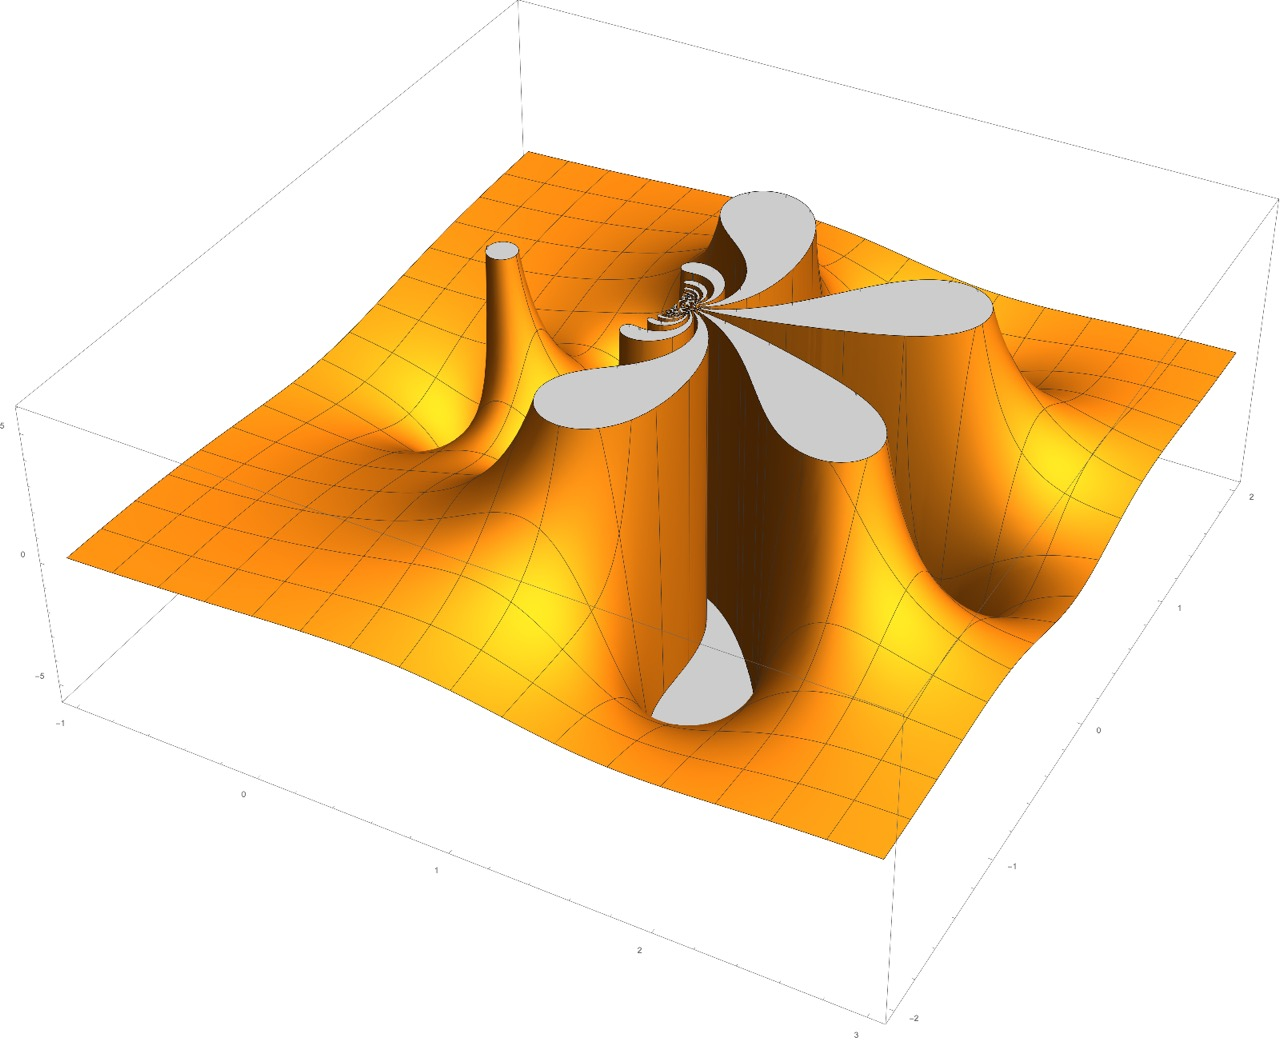
\includegraphics[height=.4\textwidth]{img/complex_f.jpg}
	\qquad 
	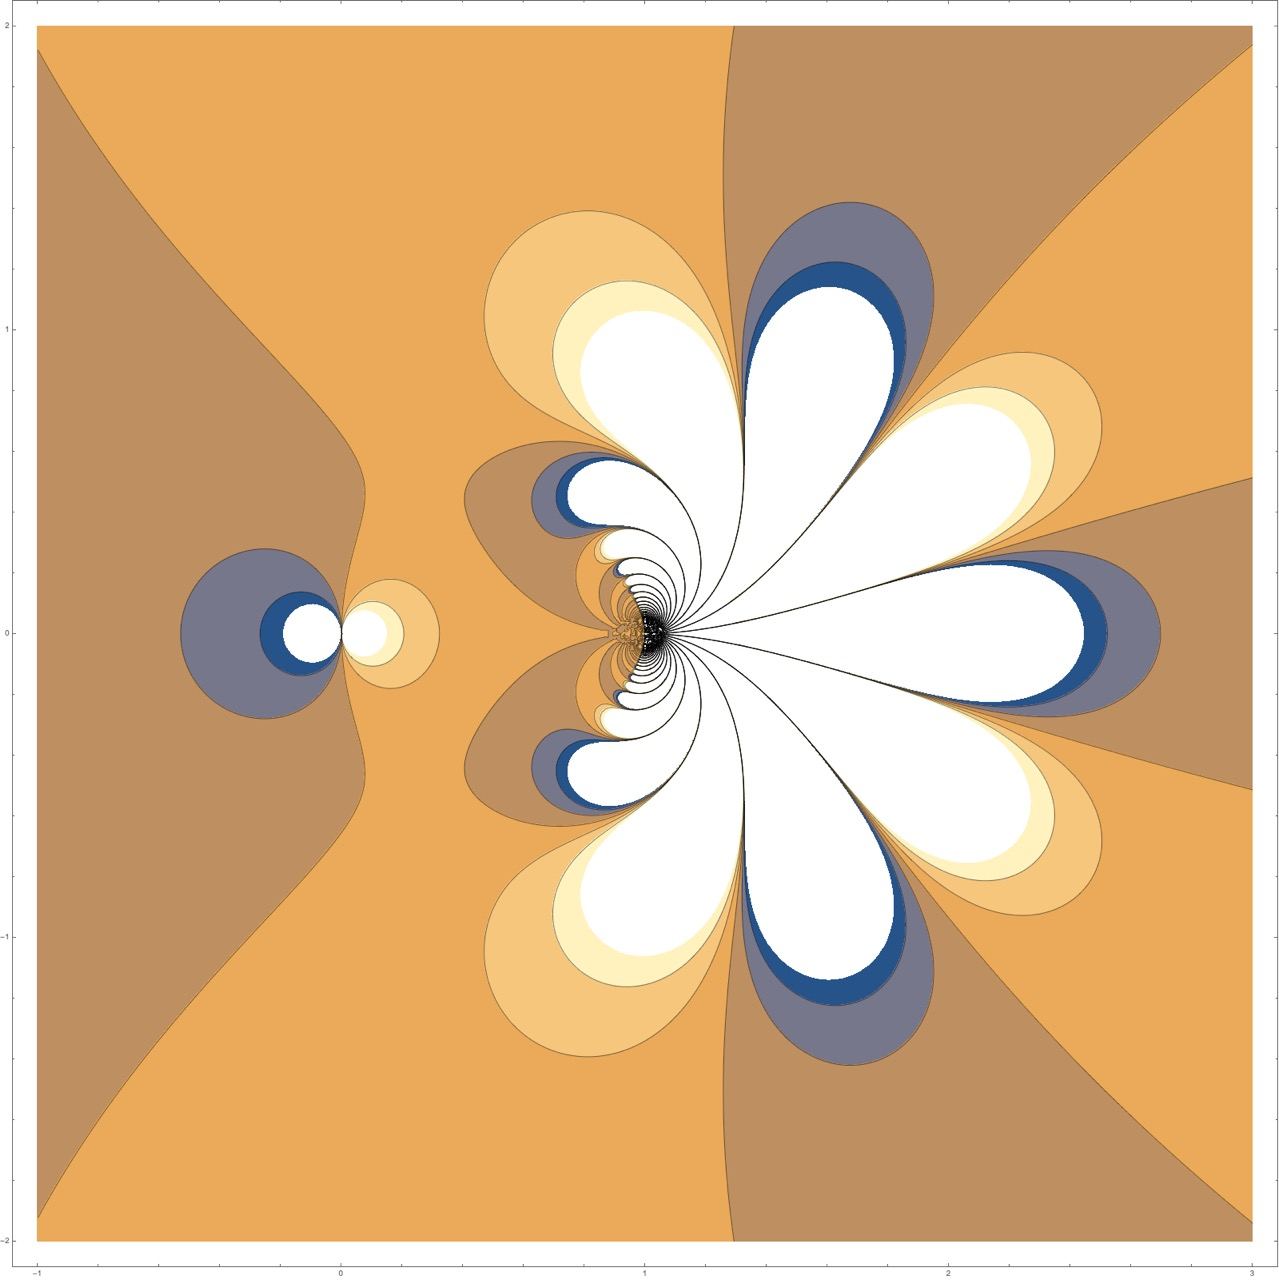
\includegraphics[height=.4\textwidth]{img/complex_f2.jpg}
	\caption{Real part of a particularly complex function (left), and 
	its contour plot (right).}
\end{figure}

\subsection*{Prerequisites}

Good command of single and multivariable calculus at the level of MATH 1310, 1320, and 2310.

\section{Necessary information}
\bigskip

\textbf{Class times:}   TuTh 12:30PM - 1:45PM in
\emph{New Cabell 309}

\medskip


\textbf{Exams:} Please do not make travel plans which conflict
with the midterms or the final exam.
\begin{itemize}
	\item \textbf{Midterm 1:} In-class on Thursday, February 6 (class time, New Cabell 309).
	\item \textbf{Midterm 2:} In-class on Tuesday, April 7 (class time, New Cabell 309).
	\item \textbf{Final exam:} Tuesday, May 5, 2-5 (New Cabell 309).
\end{itemize}

\medskip

\textbf{Instructor:} Leonid Petrov
\medskip

\textbf{Email:} \email{petrov@virginia.edu} or \email{lenia.petrov@gmail.com}
\medskip

\textbf{Office:} 209 Kerchof Hall
\medskip

% \textbf{Teaching Assistant (grader):}
% Aoran Wu, 119 Kerchof Hall, \email{aw5dk@virginia.edu}
% \medskip

\textbf{Office hours:}
TBA

You are welcome to make an appointment and meet outside the usual office hours. 
For this, please use the online tool located at
\url{https://lpetrov.cc/teaching/}. (I am automatically available during office hours --- 
and you cannot schedule appointments online for those times.)
You can make as 
many appointments as you want.

\medskip

\textbf{Course webpage:}
I will set up a collab page for homework submissions and course materials.

\section{Course materials}

The textbook is “\emph{Fundamentals of Complex Analysis}” (3rd edition)
by Saff and Snider, Pearson, ISBN-10: 0139078746.
We will discuss material from Chapters 1--6, and selected topics from Chapters 7--8.

\section{Assessing your learning}

Learning mathematics means \emph{doing} mathematics: during class meetings, on your own, and in groups. 
In this course, doing mathematics mainly amounts to solving problems. 
Below are the concrete aspects which are assessed in this course:

\subsection{Homework}

Weekly homework will consist of
problems aligned with lectures and quizzes,
to help you practice and enrich the material presented in class.
Putting an adequate effort into solving the homework
problems and
communicating your solutions clearly is
of paramount importance for your learning.
The homeworks are due \textbf{in class} on the specified date, and will be assigned at least a week before the due
date. 
Please \textbf{put your problems in order}, indicating clearly which problems you're skipping --- this will greatly help with the grading.

Homework solutions are posted soon after the
homework deadline, so late work cannot be accepted.
The lowest homework grade will be dropped.

The homeworks are graded ``coarsely'', that is,
each homework will be assigned one of four grades: 
\begin{equation*}
\begin{tabular}{l|l|l|l|l}
Grade & VG (very good) & G (good) & OK   & N \\
\hline
& \parbox{.21\textwidth}{All problems solved correctly with minor issues like arithmetic mistakes, and solutions explained
in full detail}
& \parbox{.21\textwidth}{Most problems solved correctly, and solutions explained in reasonable (close to full) detail}
& \parbox{.21\textwidth}{ {\ }\\More than $3/4$ of problems attempted, many 
solutions are incorrect, incomplete, or not explained in detail, 
but the work displays adequate understanding of most of the material\\{}}
& \parbox{.21\textwidth}{Work not submitted on time, or less than $3/4$ of problems 
attempted, or most solutions are incomplete, or work clearly displays lack of understanding of most of the material}\\
\hline
\%    & 100\%          & 90\%     & 75\% & 0\%
\end{tabular}
\end{equation*}
It is expected that most students 
who put reasonable effort into the homework
will get VG or G grades. 


% \subsection*{Homework submission guidelines --- strictly enforced}
% The homework \textbf{must be submitted only on Collab} (i.e., hard copies are not accepted).
% Take pictures or scan your work,
% make sure it's readable,
% put it into a \emph{single PDF file with correct orientation},
% and upload it before the deadline.

% Submitting work like this has many benefits:
% (1) you retain a paper copy to
% prepare for tests;
% (2) your submitted work is never misplaced or lost, and there is a digital trail;
% (3) the grading will be faster.
%
% If you have any trouble submitting homework online, ask me and I can teach you.

\subsection*{Note on collaboration on homework assignments}
\label{collaboration}

Group work on homework problems is allowed and encouraged.
Discussions are in general very
helpful and inspiring when learning mathematics.
Nevertheless, before talking to others, get well started
on the problems, and contribute your fair share to the process.

When completing the written homework assignments, everyone must write up his or her own
solutions in their own words.
It is very important that you truly understand the homework solutions you hand
in, otherwise you may be unpleasantly surprised by your in-class test results.

Needless to say that when working on in-class assignments (quizzes, tests)
you are required to work alone.

\subsection{Quizzes}

There will be short quizzes (10-15 minutes)
during the classes at random days. 
They will test the previous week's material and/or recent homework
topics. 
Quizzes are not announced in advance, and there can be two quizzes
on a given week. 

You should view quizzes as testing your “work in progress”,
which will allow me to adjust the pace of the course.
For this reason, the overall quiz grade is 
included in the same “bucket” with class participation and 
office hours discussion, see below.

\subsection{Midterm tests and the final exam}

The midterms and the final exam will feature
problems modeled after homework.
The final exam is comprehensive, with a focus on the last part
after the second midterm.

The exams will be aimed at checking not so much memorization and
routine computational skills, but rather understanding of fundamental
concepts and principles and the ability to apply the material
learned to solving various problems, including those a student might
have never seen before. A missed exam gives a score of zero, unless a
student has contacted the instructor a week in advance and agreed upon a
procedure to make it up. Under the rules of
the College, early examinations are not permitted.

\subsection{How to succeed in the course}

The best way to learn in the course is to come to all lectures, take good notes
(some notes may be provided),
ask many questions,
do all the homework problems, and express your solutions
clearly.
This will prepare you well for quizzes, midterms, and the final exam.

Mathematical questions are appreciated and encouraged any time during the
class. Please use the office hours as much as possible for additional
clarifications and occasional homework help. Remember that I am available outside 
of office hours by appointment which you can book at
\url{https://lpetrov.cc/teaching/}

\subsection{Grade distribution}

Your grade will consist of:
\begin{itemize}
	\item Homework --- 20\%, lowest homework dropped
	\item Quizzes, class participation, office hours discussion --- 15\%, one or two lowest quizzes dropped
	\item Midterms --- 15\% each
	\item Final exam --- 35\%
\end{itemize}
The score above 90\% is usually enough for an A.
The score below 50\% usually means failing.
Other factors such as in-class participation
and improvement over time may impact positively your final grade.
Excessive absence may lower the final grade.

\section{Policies}

\subsection{Laptops and smartphones}

Please do not use laptops and smartphones during the class.
You won't need them to participate in the discussions, but they may easily distract
you or other students (or me!). If you \emph{absolutely} must use a laptop
(for typing up the lecture notes), please sit in the back row.

\subsection{Late/make up work} Each assignment will have due date and time.
Late assignments are not accepted. There will also be no make ups for the midterm tests and the final exam.
However, if you have special needs, emergency, or unavoidable conflicts, please
let me know as soon as possible, so we can arrange a workaround.

\subsection{Honor Code} The University of Virginia Honor Code applies to this
class and is taken seriously. Collaboration on homework
assignments is allowed within the bounds discussed above
in the corresponding section.
Any honor code violations will be referred to the
Honor Committee.

\subsection{Special needs}

All students with special needs requiring accommodations should present the
appropriate paperwork from the Student Disability Access Center (SDAC). It is
the student's responsibility to present this paperwork in a timely fashion and
follow up with the instructor about the accommodations being offered.
Accommodations for test-taking (e.g., extended time) should be arranged at
least 5 business days before an exam.




\end{document}
